% ==============================================================================
% EDITORIAL FRONT COVER (TECHNICAL REFERENCE / NATURALIST ENGRAVING)
% "Linux Forensics: A Real Case" - Alexis Real Santillán
% ==============================================================================
\begin{titlepage}
\thispagestyle{empty}

\begin{tikzpicture}[remember picture, overlay]
    % Editorial color palette
    \definecolor{coverred}{RGB}{185, 28, 28}       % Classic technical series red
    \definecolor{covergray}{RGB}{75, 85, 99}       % Neutral gray for metadata
    \definecolor{coverborder}{RGB}{229, 231, 235}  % Subtle gray border
    \definecolor{ribbonbg}{RGB}{243, 244, 246}     % Light background for ribbon

    % Pure white background
    \fill[white] (current page.south west) rectangle (current page.north east);

    % Top red bar across entire page
    \fill[coverred] (current page.north west) rectangle ($(current page.north east) + (0, -4.5mm)$);

    % --------------------------------------------------------------------------
    % DIAGONAL "SECOND EDITION" RIBBON (TOP RIGHT CORNER)
    % --------------------------------------------------------------------------
    \begin{scope}
        \clip ($(current page.north east) + (-55mm, 0)$) -- ($(current page.north east) + (0, -55mm)$) -- (current page.north east) -- cycle;
        \fill[ribbonbg] ($(current page.north east) + (-60mm, 0)$) -- ($(current page.north east) + (0, -60mm)$) 
            -- ($(current page.north east) + (0, -25mm)$) -- ($(current page.north east) + (-25mm, 0)$) -- cycle;
        \draw[coverborder, line width=0.6pt] ($(current page.north east) + (-55mm, 0)$) -- ($(current page.north east) + (0, -55mm)$);
        \draw[coverborder, line width=0.6pt] ($(current page.north east) + (-26mm, 0)$) -- ($(current page.north east) + (0, -26mm)$);
        \node[rotate=-45, text=black!85, font=\fontsize{7.5}{9.5}\selectfont\sffamily\bfseries] 
            at ($(current page.north east) + (-20mm, -20mm)$) {Second Edition};
    \end{scope}

    % Top left series badge
    \node[anchor=north west, align=left] 
        at ($(current page.north west) + (20mm, -13mm)$) {
        {\fontsize{9}{11}\selectfont\sffamily\bfseries\color{coverred} Real Production Case} \quad
        {\fontsize{9}{11}\selectfont\sffamily\color{black!30} $\vert$} \quad
        {\fontsize{8.5}{11}\selectfont\sffamily\color{covergray} Linux Digital Forensics}
    };

    % --------------------------------------------------------------------------
    % TITLE AND SUBTITLE BLOCK
    % --------------------------------------------------------------------------
    \node (covertitle) [anchor=north west, align=left, text=black, font=\fontsize{29}{35}\selectfont\sffamily\bfseries] 
        at ($(current page.north west) + (20mm, -25mm)$) {
        Linux forensics:\\[3pt]
        a real case
    };

    % Crimson separator rule
    \draw[line width=2.0pt, draw=coverred] 
        ($(covertitle.south west) + (0, -4mm)$) -- ++(32mm, 0);

    % Subtitle
    \node (coversubtitle) [anchor=north west, align=left, text width=142mm, text=black!90, font=\fontsize{10.5}{15}\selectfont\sffamily] 
        at ($(covertitle.south west) + (0, -9mm)$) {
        \textbf{Autopsy of a Cyberattack on Live Production Servers}\\[2.5pt]
        {\fontsize{9}{13}\selectfont\color{covergray} Timeless Unix/Linux fundamentals, volatile memory, and forensic correlation}
    };

    % --------------------------------------------------------------------------
    % CENTRAL ARTWORK: COLOR NATURALIST ENGRAVING (BLOODHOUND)
    % --------------------------------------------------------------------------
    \node (artnode) [anchor=center, inner sep=0pt] 
        at ($(current page.center) + (0, -14mm)$) {
        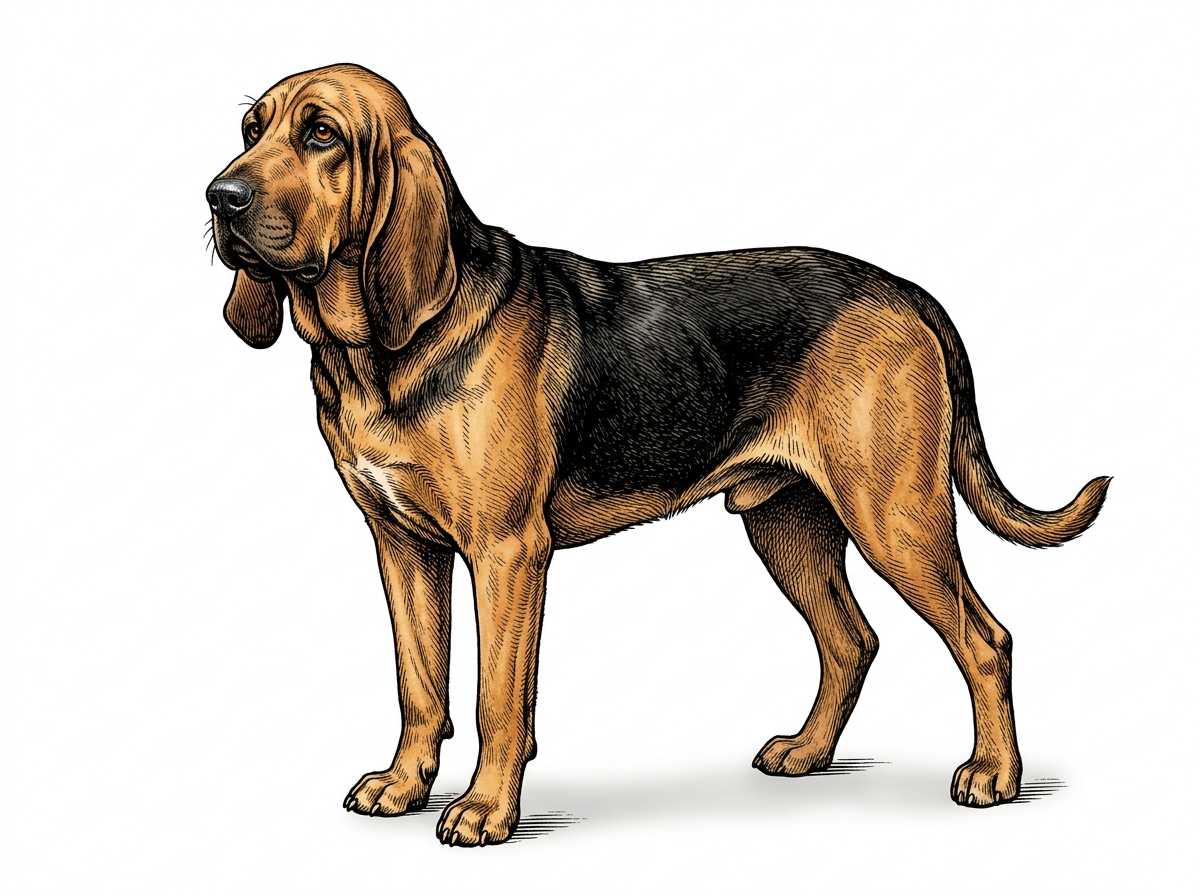
\includegraphics[width=13.0cm, height=13.0cm, keepaspectratio]{figures/sabueso_color.jpg}
    };

    % --------------------------------------------------------------------------
    % FOOTER: AUTHOR BLOCK
    % --------------------------------------------------------------------------
    \draw[coverborder, line width=0.6pt] 
        ($(current page.south west) + (20mm, 26mm)$) -- ($(current page.south east) + (-20mm, 26mm)$);

    \node[anchor=south east, align=right] 
        at ($(current page.south east) + (-20mm, 12mm)$) {
        {\fontsize{13.5}{16}\selectfont\sffamily\bfseries\color{black} Alexis Real Santillán}\\[3pt]
        {\fontsize{9}{12}\selectfont\sffamily\color{covergray} Infrastructure \& Cybersecurity Consultant}
    };

\end{tikzpicture}

\newpage
\thispagestyle{empty}
\mbox{}
\newpage

% ==============================================================================
% HALF-TITLE / INNER TITLE PAGE
% ==============================================================================
\thispagestyle{empty}
\begin{center}
    \vspace*{1.2cm}

    {\fontsize{9}{12}\selectfont\sffamily\bfseries\color{secondary} INCIDENT RESPONSE METHODOLOGY AND FORENSIC REPORT}\\[0.8cm]

    {\fontsize{26}{30}\selectfont\sffamily\bfseries\color{primary} Linux forensics:}\\[0.3cm]
    {\fontsize{22}{26}\selectfont\sffamily\bfseries\color{primary} a real case}\\[0.8cm]

    {\large\textsf{\textbf{Autopsy of a Cyberattack on Live Production Servers}}}\\[0.4cm]
    {\normalsize\textsf{Incident response, volatile memory, and multi-system event correlation}}\\[0.8cm]

    {\small\textsf{\textit{The enduring power and maturity of foundational Unix/Linux tools against modern threats}}}\\[1.2cm]

    {\large\textsf{\textbf{Second Edition}}}\\[1.4cm]

    \rule{0.35\textwidth}{1.0pt}\\[1.6cm]

    {\Large\textbf{Alexis Real Santillán}}\\[0.4cm]
    {\large Infrastructure and Cybersecurity Consultant}\\[0.2cm]
    {\normalsize\textsf{Linux Open Source de México}}\\[2.2cm]

    \vfill

    {\small\textsf{Technical forensic report adapted for defensive security and digital investigations}}\\[0.2cm]
    {\footnotesize\textsf{Author contact: \texttt{alexisreal@gmail.com} $\;\vert\;$ \texttt{linuxopensource.org}}}

\end{center}
\end{titlepage}
